\documentclass[t]{beamer}
\usepackage{listings}
\usepackage{minted}

\usetheme{default}
\usebackgroundtemplate{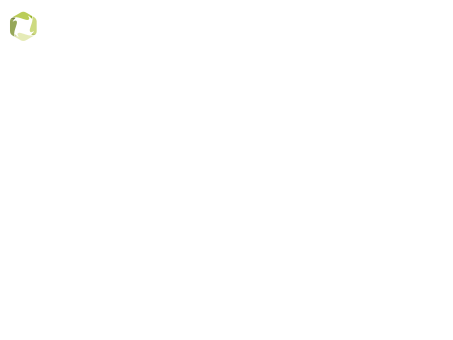
\includegraphics[width=\paperwidth]
                                       {../cpeb_bkground_topleftlogo.pdf}}

\setbeamertemplate{frametitle}{
  \centering\vspace{1mm}\insertframetitle\par\vspace{3mm}
}

\usepackage[style=nature,
            hyperref,
            backend=biber,
            isbn=false,
            doi=false,
            url=false,
            date=year,
            maxbibnames=3
           ]{biblatex}

\bibliography{kwip-tic.bib}

\title{\texttt{kWIP}: The k-mer Weighted Inner Product}
\author{Kevin Murray}
\institute{Borevitz Lab, CPEB, ANU}
\date{21 August 2015}

\begin{document}

{
\usebackgroundtemplate{
\includegraphics[width=\paperwidth]{../cpeb_bkground_centered.pdf}}
\begin{frame}
  \titlepage
  \vfill
\end{frame}
}

\begin{frame}{Disclaimer}
  \begin{center}
    \vfill
    \texttt{DRAFT}
    \\
    \pause
    \small{Or as Norman says, \texttt{kWIP} is Kevin's Work In Progress}
    \vfill
  \end{center}
\end{frame}


\begin{frame}{Collaboration}
  \begin{itemize}
    \item This work is a collaborative effort
      \begin{itemize}
        \item Norman Warthmann
        \item Cheng Soon Ong
        \item Chris Webers
      \end{itemize}
  \end{itemize}
\end{frame}

\begin{frame}{Overview}
  \begin{itemize}
    \item Motivation
    \item Technological overview
    \item Early results and plans
    \item Demonstration
  \end{itemize}
\end{frame}

\begin{frame}{Large-scale population genomics}
  \begin{itemize}
    \item Moving from 100s to 1000s and 10000s of samples \textit{per PhD!}
      \pause
    \item Efficient algorithms to analyse large-scale genomic data
    \begin{itemize}
      \item Reference \& alignment free: \textit{less bias, de novo}
      \item Platform/protocol agnostic: \textit{future proof}
      \item Computationally efficient: \textit{not the bottleneck}
      \item Cross scale: \textit{one tool to rule them all}
    \end{itemize}
  \end{itemize}
  \begin{center}
    \includegraphics[width=\textwidth]{img/cross-scale.png}
  \end{center}
  \tiny{after \textcite{peterson_double_2012}}
\end{frame}


\begin{frame}{Rapid and Basic Clustering}
  \begin{itemize}
    \item Rough approximation of sample relatedness required
    \item Enables a ``zooming'' approach to genetic analysis
    \item Required for population resampling
  \end{itemize}
  \pause
  \begin{center}
    \includegraphics<1>[width=\textwidth]{img/restruct-1}
    \includegraphics<2>[width=\textwidth]{img/restruct-2}
    \includegraphics<3>[width=\textwidth]{img/restruct-3}
    \includegraphics<4>[width=\textwidth]{img/restruct-4}
  \end{center}
  \tiny{after \textcite{brachi_genome-wide_2011}}
\end{frame}

\begin{frame}{\textit{De novo} technical control}
  \begin{itemize}
    \item Sample DNA not very physically distictive
      \begin{itemize}
        \item Mix-ups and contamination occur
      \end{itemize}
    \item Catching mix-ups early important
      \begin{itemize}
        \item Not just for your own data: SRA not so perfect
      \end{itemize}
  \end{itemize}
  Ath 80 FIGURE HERE % TODO
\end{frame}

\begin{frame}{Technological Overview}
  \begin{itemize}
    \item $k$-mer analysis
    \item Hashing and Probablistic Data Structures
    \item Population and RunFrequency Hashes
    \item (Weighted) Inner Products
  \end{itemize}
\end{frame}

\begin{frame}{$k$-mer analysis}
  \begin{columns}[t]
    \column{0.6\textwidth}
      \begin{itemize}
        \item<1-> Analyse $k$-length words of sequences
        \item<2> Computationally and biologically appropriate
        \begin{itemize}
          \item<2> Fast
          \item<2> Constant-memory (using \texttt{khmer})
          \item<2> Scalable and parallelisable
          \item<2> Cross-scale
        \end{itemize}
      \end{itemize}
      \vfill
    \column{0.4\textwidth}
    $k = 3$\\
    \texttt{ACGTGT}\\
    \texttt{ACG~~~}\\
    \texttt{~CGT~~}\\
    \texttt{~~GTG~}\\
    \texttt{~~~TGT}
  \end{columns}
\end{frame}

\begin{frame}{Hashes and Hash Functions}
  \begin{itemize}
    \item Hash function e.g. \mint{python}|hash('ACG') => 5234315134|
      \pause
    \item ``Hash'': a probablistic data structure
      \begin{itemize}
        \item Constant memory
        \item Easy set operations and inner product
        \item Implicit de Bruijn graph
        \item Implemented in C Titus Brown's \texttt{khmer}
        \item AKA Countgraph
      \end{itemize}
  \end{itemize}
\end{frame}

\begin{frame}{Hash}
  \begin{itemize}
    \item Vector of large prime length (e.g. 1e9 + 7)
    \item Indexed modulo length $(bin = h(w_i) \mod prime)$
  \end{itemize}
  \begin{center}
    \includegraphics<1>[width=0.6\textwidth]{img/hash-0.png}
    \includegraphics<2>[width=0.6\textwidth]{img/hash-1.png}
    \includegraphics<3>[width=0.6\textwidth]{img/hash-2.png}
    \includegraphics<4>[width=0.6\textwidth]{img/hash-3.png}
    \includegraphics<5>[width=0.6\textwidth]{img/hash-4.png}
  \end{center}
\end{frame}


\begin{frame}{Hash Operations}
  \begin{itemize}
    \item Population sum, or hash frequency
  \end{itemize}
  \begin{center}
    \includegraphics<1>[width=0.6\textwidth]{img/hash-sums.png}
    \includegraphics<2>[width=0.6\textwidth]{img/hash-sumfreq.png}
  \end{center}
\end{frame}

\begin{frame}{$k$-mer based clustering}
  \begin{itemize}
    \item Alignment-free sequence clustering is a whole field
    \item $D2$ and friends
    \item Most require sequence gene/genome
    \item Many use inner product as similarity measure
  \end{itemize}
  \begin{center}
    \includegraphics[width=0.6\textwidth]{img/foret-et-al-d2.png}
  \end{center}
\end{frame}

\begin{frame}{Shannon Entropy}
  \begin{itemize}
    \item Measure of Information
    \item $ -\sum\limits_{i} p_i log(p_i) $
  \end{itemize}
  \begin{center}
    \includegraphics[width=0.6\textwidth]{img/shanent.pdf}
  \end{center}
\end{frame}

\begin{frame}{\texttt{kWIP}}
  \begin{itemize}
    \item The $k$-mer Weighted Inner Product
      \begin{itemize}
        \item Extends alignment-free seq comparison to raw NGS data
      \end{itemize}
    \pause
    \item Algorithm:
      \begin{itemize}
        \item For each sample: count all $k$-mers into a Hash
        \pause
        \item For each analysis set, i.e ``population'':
          \begin{itemize}
            \item Calculate the informational entropy of hash frequency ($H$)
            \item For each pair of samples $A$ and $B$, calculate \\
              $\sum^{n}_{i=0} A_i \cdot B_i \cdot H_i$
          \end{itemize}
      \end{itemize}
  \end{itemize}
  \begin{center}
    \includegraphics[width=0.4\textwidth]{img/hash-wip.png}
  \end{center}
\end{frame}


\begin{frame}{\texttt{kWIP}}
  \begin{itemize} % TODO: columns
    \item The software:
      \begin{itemize}
        \item \texttt{C++}, $>$2000 lines of code
        \item Uses \texttt{khmer} for $k$-mer counting \& hashing
        \item Parallelised, $\approx$ 10 hrs for 96 rice samples.
        \item GNU GPL licensed, source code on GitHub
      \end{itemize}
      \begin{center}
        \includegraphics[width=0.5\textwidth]{img/kwip-doc-screenshot.png}
      \end{center}
  \end{itemize}
\end{frame}

\begin{frame}{\texttt{kWIP} Experiments}
  \begin{itemize}
    \item 3000 rice genomes:
      \begin{itemize}
        \item 3000 rice lines from known families
        \item Analysing in sets of $\approx 100$, from all major groups
        \item Recover known grouping w/ \texttt{kWIP}, not w/ unweighted IP
        \item Sensitive to read depth
      \end{itemize}
    \item Simulation
      \begin{itemize}
        \item Fake population genome sequencing studies
      \end{itemize}
  \end{itemize}
\end{frame}

\begin{frame}{96 Rice Runs}
  \begin{itemize}
    \item Set of 96 rice runs from 12 samples (8 tech reps)
    \item 6 samples each from 2 major groups (Indica, Japonica)
    \item Expectations:
      \begin{itemize}
        \item All runs cluster into groups of 6 reps (12 samples)
        \item Big split between two groups: 6 samples each
      \end{itemize}
    \item We see this with \texttt{kWIP}, not with Unweighted IP
  \end{itemize}
\end{frame}

\begin{frame}
  \begin{center}
    \includegraphics<1>[width=\textwidth]{img/distmat-both.png}
    \includegraphics<2>[width=\textwidth]{img/dendro-both.png}
  \end{center}
\end{frame}

\begin{frame}
  \begin{center}
    \includegraphics<1>[width=0.6\textwidth]{img/dendro-wip.png}
    \includegraphics<2>[width=0.6\textwidth]{img/dendro-ip.png}
  \end{center}
\end{frame}


\begin{frame}{Simulation}
  \begin{itemize}
    \item Now for an Jupyter notebook
  \end{itemize}
\end{frame}

\begin{frame}{Thanks}
  \begin{itemize}
    \item My collaborators: Cheng Soon Ong, Christfried Webers, Norman Warthmann
    \item \{Super,Ad\}visors: Justin, Sylvain, Gavin and Barry
    \item \texttt{khmer} folks: C. Titus Brown, Michael Crusoe, Camille Scott (DIB-lab) @ UC Davis
    \item Yourselves
  \end{itemize}
\end{frame}

\begin{frame}[shrink=20]{References}
  \printbibliography
  \vfill
  .
\end{frame}


\begin{frame}{Missing heritability in the field?}
  \begin{itemize}
    \item Find more diversity in the field!
    \item Sample natural populations
      \begin{itemize}
        \item Ecological hypotheses of trait selection, adaptation
        \item Sample widely as possible across non-uniform genetic diversity
      \end{itemize}
      \pause
    \item Now \textbf{complexity limited}: complex kinship \& population
      structure
    \item Mandates development of economic, accurate large scale population
      genomics
  \end{itemize}
  \begin{center}
    \includegraphics[width=\textwidth]{img/jared-tree.pdf}
  \end{center}
\end{frame}

\end{document}
